\documentclass[a4paper]{article}
\usepackage[top=1in,bottom=1in,left=1in,right=1in]{geometry}
\usepackage[utf8]{inputenc}
\usepackage{amsmath}
\usepackage{amssymb}
\usepackage{setspace}
\usepackage{color}
\usepackage{graphicx}
\usepackage{subcaption}
\graphicspath{ {../figures/} }

\newcommand{\Rbb}{\mathbb{R}}
\newcommand{\Expect}{\mathbb{E}}



\title{Temp}
\author{Runjing Liu}
\date{\today}

\begin{document}

\maketitle


{Dimensionality reduction on roll call vote data in the House of Representatives in the 110th Congres. (a) Nonnegative matrix factorization on the $448\times 1707$ matrix (448 representatives, 1707 bills) of roll call votes into two matrices of dimensions $448\times 2$ and $2\times 1707$. The rows of the $448\times 2$ matrices were plotted to visualize the distribution of representatives in a 2D space, and we clearly see division along party lines. (b) Principle component analysis on the roll call vote data. The eigenvalues and eigenvectors of the $448\times 448$ covariance matrix of representative voting data were computed, and each representative's voting profile was projected onto the space of the two eigenvectors with the two largest eigenvalues.}


We chose to model caucus memberships because initial exploratory data analysis suggested that caucus memberships are related to a legislator's voting behavior. Figure \ref{fig:VotesVsCaucus} plots the number of shared caucuses between two representatives against the proportion of bills on which they voted the same way, and we see that the more caucuses two members share, the more likely they are to vote the same way. 

\begin{figure}[h]
  \centering
        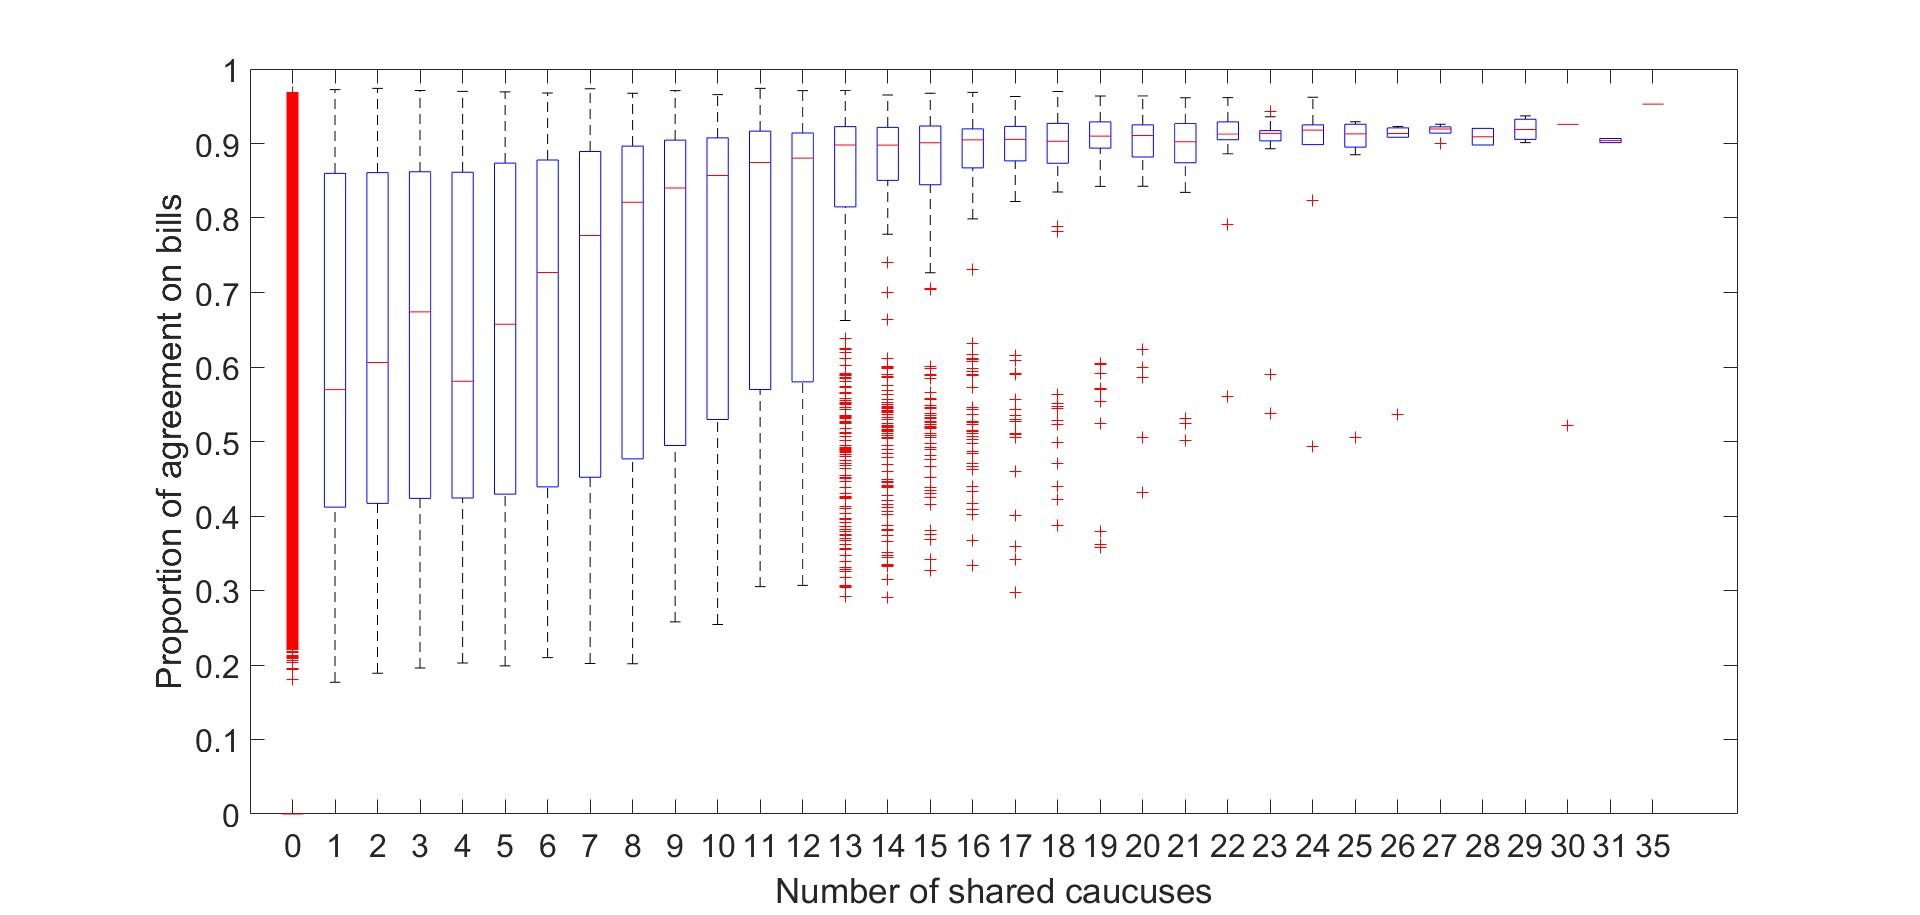
\includegraphics[width=\textwidth]{Caucus_vs_Votes.jpg}
  \caption{The distribution of agreement on bills as a function of the number of caucuses two representatives share. We see that the more caucuses people share, the more likely they are to agree on a bill. }
          \label{fig:VotesVsCaucus}
\end{figure}


Figure \ref{fig:Nhood_Caucus} shows the relationship between representatives within several caucuses in an undirected graphical model. We first used roll call vote data to infer the graph structure among the representatives in the entire House; we assumed pairwise interactions described via an Ising model in which each node denotes a binary variable of a representative voting either yes or no. The edges were inferred using neighborhood selection \cite{Hastie2015}, and the graphs shown in figure \ref{fig:Nhood_Caucus} are subsets of this full graph corresponding to members of a caucus. The connectivity (measured by the fraction of total edges present) of the full graph with 448 representatives is 0.064, while the connectivity within the caucus subgraphs was much higher. This suggests that a representative is more likely to be influenced by a member of his or her caucus than another random representative in the House.\par

Therefore, this strongly motivates taking into account interactions among the representatives in Congress. In particular, this analysis suggests that caucus memberships may at least partly explain whether two representatives will vote in a similar fashion. Therefore, we proceed in this project by utilizing caucus membership data and connecting them to ideal points using a stochastic block model; specifically, we hope that caucus memberships will inform a latent community structure among the representatives, and exploiting these interactions, we obtain better predictions of ideal points and hence better predictions of roll call votes. 

\begin{figure}[h]
  \centering
    \begin{subfigure}[b]{0.49\textwidth}
        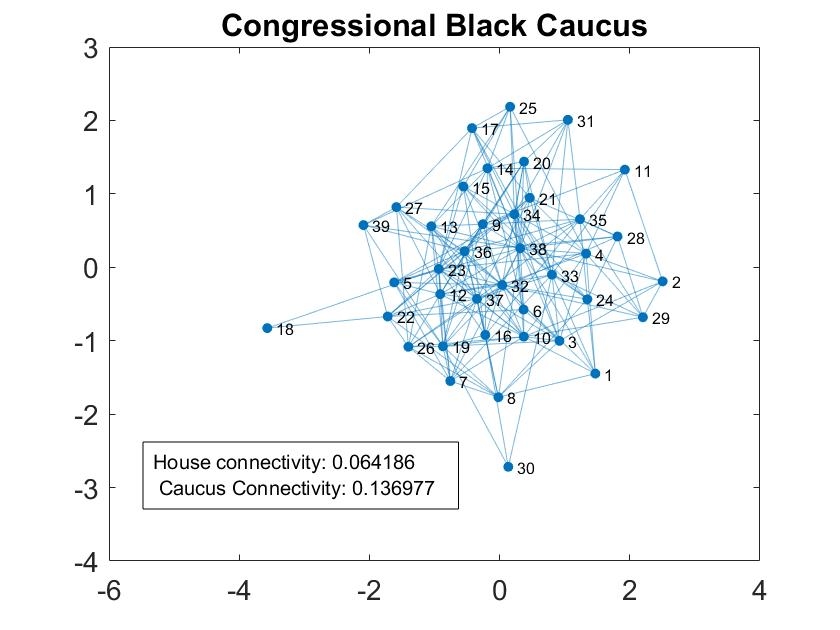
\includegraphics[width=\textwidth]{/Neighborhood_Regression/Congressional_Black_Caucus.jpg}
        \caption{}
    \end{subfigure}
          \begin{subfigure}[b]{0.49\textwidth}
        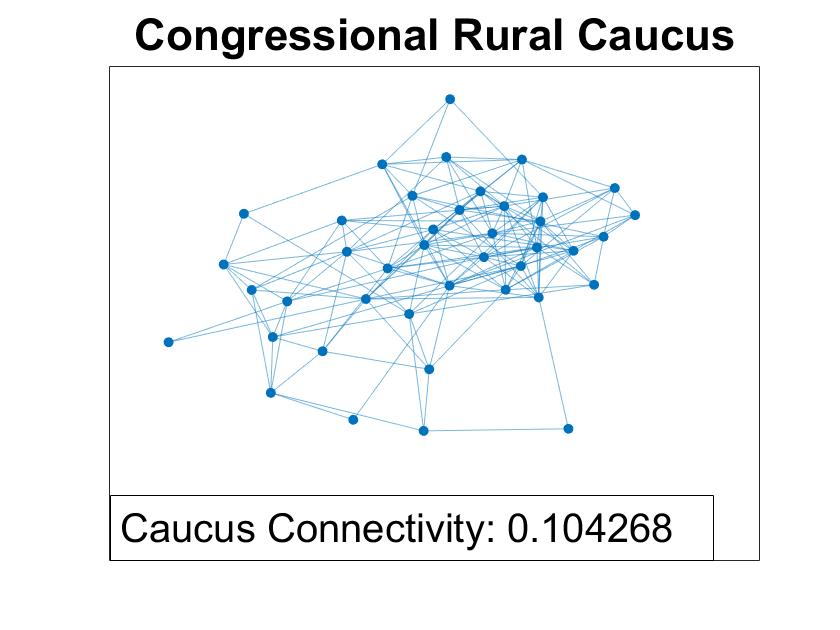
\includegraphics[width=\textwidth]{/Neighborhood_Regression/Congr_Rural_Caucus.jpg}
        \caption{}
    \end{subfigure}
        \begin{subfigure}[b]{0.49\textwidth}
        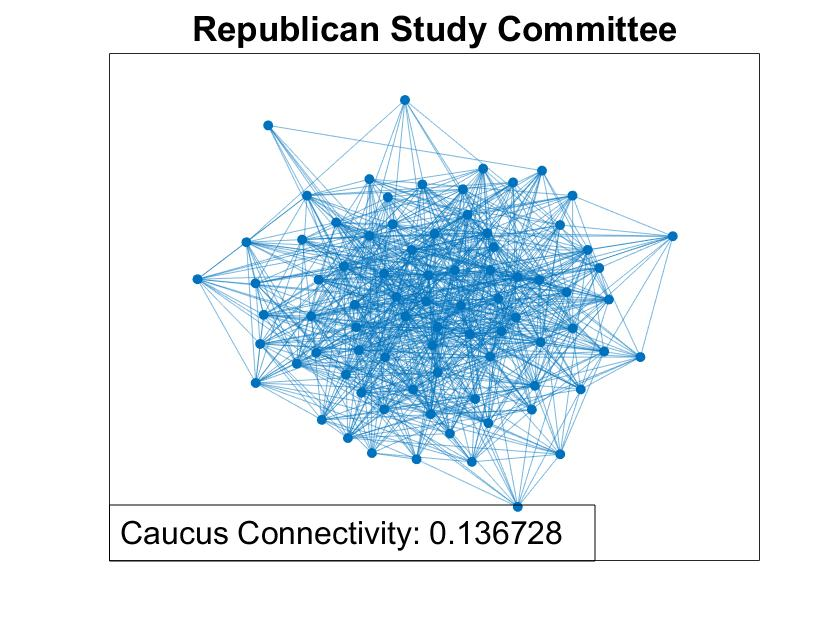
\includegraphics[width=\textwidth]{/Neighborhood_Regression/Rep_Study_Committee.jpg}
        \caption{}
    \end{subfigure}
          \begin{subfigure}[b]{0.49\textwidth}
        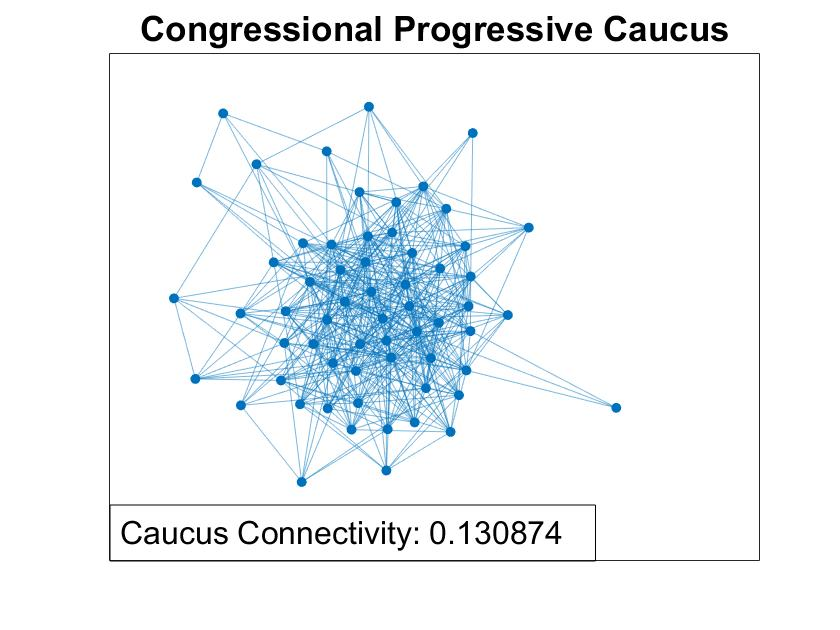
\includegraphics[width=\textwidth]{/Neighborhood_Regression/Congr_Prog_Caucus.jpg}
        \caption{}
    \end{subfigure}
  \caption{Neighborhood regression on roll call vote data was used to infer an undirected graphical model capturing relationships among all members of the House of Representatives. Each node represents a random variable corresponding to a legislator voting ``yea'' or ``nay'' on a bill, and we assumed pairwise interactions using an Ising model. Shown here are subgraphs with representatives taken from a given caucus. The caucuses are their connectivities shown here are (a) the Congressional Black Caucus, connectivity 0.137; (b) the Congressional Rural Caucus, connectivity 0.104; (c) the Republican Study Committee, connectivity 0.136; and (d) the Congressional Progressive Caucus, connectivity 0.131. In each case, the connectivity within the caucuses was higher than the connectivity of the full House (0.064).}
      \label{fig:Nhood_Caucus}
\end{figure}


\section{Conclusions and Future directions} 
While LC-IPM offers similar predictive performance to the standard ideal point model, we gain the ability to detect more subtle clusters within and between the two large party clusters. This ability to analyze the social network among members of Congress is of particular interest to political scientists. \par

Moreover, by taking into account caucus data, we can still make reasonable predictions for junior representatives for whom we do not have extensive vote data.  {\color{red} Eli will add to this}  \par

Finally, a key advantage to our generative model is its modularity, and in future work we would be interested in the composability of hierarchical models from multiple data sources. While this project incorporated caucus data to better inform estimates for the representatives' ideal points, another direction to explore would be to utilize data on bills to better estimate their difficulty and discrimination. For example, we may follow the example in \cite{Gerrish2011} to combine LC-IPM with supervised topic modeling and infer the latent topics in a bill from a bill's text; these latent topics then inform a bill's difficulty and discrimination. On the other hand, we may also explore incorporating legislators' speech transcripts in deliberating the bill (\cite{Quinn2006}, \cite{Thomas2006}). Our model could also be augmented by incorporating bill metadata (like sponsorships), or legislator metadata (like ethnicity or state). \par

Overall, LC-IPM connects voting data to caucus memberships, and enables us to analyze how a social network influence legislative results. While we were motivated by congressional data, our model also applies to more general collaborative filtering settings with relational data.


%We have developed several models associating the text
%of legislation to legislators’ voting patterns. These
%models provide a way of exploring large collections of
%legislative data and predicting the votes of new bills.
%Though we were motivated by (and focused on) political
%science data, we note that these models are among
%several (as, e.g., (Agarwal & Chen, 2010)) that can be
%applied in a variety of collaborative filtering settings.
%They provide a way to model a collection of users and
%their decisions about collections of textual items.

%One of the central advantages of generative probabilistic
%models is their modularity. Another avenue
%of future work is to incorporate other elements of the
%legislative process, such as speech transcripts (Quinn
%et al., 2006; Thomas et al., 2006) and auxiliary features
%such as bill sponsor, into this model’s supervision,
%to improve both the predictive power and exploratory
%capabilities of the ideal point topic model.
%
%We are also interested in the composability of hierarchical models for multiple data sources. 
%





\end{document}